\documentclass[compress,10pt]{beamer}
% version imprimable pour assistance
%\documentclass[10pt, green, handout]{beamer}
\usepackage[T1]{fontenc}
\usepackage[utf8]{inputenc}
\usepackage[frenchb]{babel} % le document est en français
\usepackage{rotating,amsmath}
\usepackage{graphicx,cancel}       % pour ins\'erer des figures
        % pour d\'efinir plus de couleurs
\usetheme{Malmoe}  %Applique le theme INRA (ce dernier doit être present dans le repertoire courant)
\usepackage{xcolor,colortbl}
\usepackage{array}
\usepackage{mdframed}

\usepackage{lmodern}	
\usepackage{tikz}
\usetikzlibrary{positioning,shapes,arrows}


\definecolor{dgreen}{RGB}{102,193,191}
\definecolor{lgreen}{RGB}{0,140,142}
%\setbeamercolor{structure}{fg=INRA@dinst}

\setbeamertemplate{blocks}[rounded][shadow=true]
\setbeamercolor{block title}{use = structure , fg=dgreen, bg = dgreen!35}
\setbeamercolor{normal text}{fg=black,bg=white}
\setbeamercolor{alerted text}{fg=lgreen}
\setbeamercolor{example text}{fg=lgreen}
\setbeamercolor{structure}{fg=dgreen} %d'où ce bleu par défaut
\setbeamercolor{background canvas}{parent=normal text}


 \usepackage{tikz}

\usetikzlibrary{calc,shapes,backgrounds,arrows,automata,shadows,positioning}



\addtobeamertemplate{navigation symbols}{}{%
    \usebeamerfont{footline}%
    \usebeamercolor[fg]{footline}%
    \hspace{1em}%
    \insertframenumber/\inserttotalframenumber
}
%\pgfdeclareimage[height=\paperheight,width=\paperwidth]{intro}{plots/plante-insecte-ombre-COLLAGE.jpg}
%\setbeamertemplate{background canvas}{\pgfuseimage{intro}}

%\newmdenv[tikzsetting={draw=black, fill=white, fill opacity =0.7, line width= 4pt}, backgroundcolor=white, leftmargin=0, rightmargin=40,innertopmargin=4pt]{titlebox}


\setbeamertemplate{frametitlecontinuation}{\insertcontinuationcountroman}

%-------------------------------------------------------------------------------
% Quelques options pdf
%-------------------------------------------------------------------------------
\hypersetup{
pdfpagemode = FullScreen, % afficher le pdf en plein \'ecran
pdfauthor   = {},%
pdftitle    = {},%
pdfsubject  = {},%
pdfkeywords = {Science,Impact},%
pdfcreator  = {PDFLaTeX,emacs,AucTeX},%
pdfproducer = {INRA}%
}


\newcommand\Wider[2][3em]{%
\makebox[\linewidth][c]{%
  \begin{minipage}{\dimexpr\textwidth+#1\relax}
  \raggedright#2
  \end{minipage}%
  }%
}

\AtBeginSection[]
{  \begin{frame}
  \frametitle{}
  \tableofcontents[currentsection, hideothersubsections]
  \end{frame} 
}



%
\newcommand{\bX}{\boldsymbol{X}}

\newcommand{\Xall}{\bX}
\newcommand{\Zall}{\bZ}
\newcommand{\M}{\mathcal{M}_{K_0,K_1,\dots, K_Q}}
\newcommand{\ind}{\mathds{1}}

\newcommand{\Mcal}{\mathcal{M}}


\newcommand{\bZ}{\boldsymbol{Z}}
\newcommand{\bpi}{\boldsymbol{\pi}}
\newcommand{\balpha}{\boldsymbol{\alpha}}
\newcommand{\btau}{\boldsymbol{\tau}}


\def\Ecal{\mathcal{E}}



\def\N{\mathbb{N}}
\def\R{\mathbb{R}}
\def\F{\mathcal{F}}
\def\Nb{\boldsymbol{N}}
\def\bZ{\boldsymbol{Z}}
\def\btheta{\boldsymbol{\theta}}
\def\bpi{\boldsymbol{\pi}}
\def\bY{\boldsymbol{Y}}
\def \ind{\mathbb{I}}
\def \P{\mathbb{P}}
\def \vert{\color{dgreen}}

\def \rouge{\color{red}}
\def \noir{\color{black}}
%-------------------------------------------------------------------------------
\title[Complex networks]{Analysis of complex networks}
 
%\subtitle{Presentation Soustitre}sp

\author{Sophie Donnet, MIA Paris, INRAE }

 
\date{Update:  \today}
 

%-F1------------------------------------------------------------------------------

\begin{document}
%-------------------------------------------------------------------------------------

\begin{frame}
\titlepage

\vspace{-.5cm}

\includegraphics[scale=.1]{plots/AgroParisTech_-_logo.PNG}
\vspace{-1.2cm}
\begin{flushright}
 
\includegraphics[scale=.3]{plots/Logo-INRAE.jpg}
 \end{flushright}

\end{frame}


\setbeamertemplate{background canvas}[default]

\section[Contexte]{Introduction}

%-------------------------------------------------------------------------------

\begin{frame}{From simple and bipartite networks... }

\begin{itemize}
\item SBM and LBM : probabilistic models for simple and bipartite networks.
\item The SBM involves  on group of nodes : we obtain a clustering based on the observation of their interactions.
\item The LBM involves  two groups of node  : we obtain a bi- clustering based on the bipartite network. 
\end{itemize}

\end{frame}






%-------------------------------------------------------------------------------
\begin{frame}{... to more complex networks}

Sometimes, we would like to study some more complex networks... 
For instance : 
\begin{itemize}
\item  study several types of relations at the same time
\item study tripartite or more complex networks... 
\item study at the same time the relations between individuals and the connexions between the organizations they belong to. 

\end{itemize}
 

\end{frame}

%-------------------------------------------------------------------------------

\section{Multiplex networks}

\begin{frame}{Multiplex networks}

\begin{block}{Definition}
Given a set of vertices, we speak of a multiplex network if we study several relations simultaneously. 
\end{block}
\vspace{2em}

\begin{columns}
\begin{column}{0.5\textwidth}
\textbf{Example} : 
\begin{itemize}
\item Vertices :  students
\item Network  1:    facebook 
\item Network  2:    LinkedIn 
 \end{itemize}
\end{column}
\begin{column}{0.5\textwidth} 
 \begin{center}
  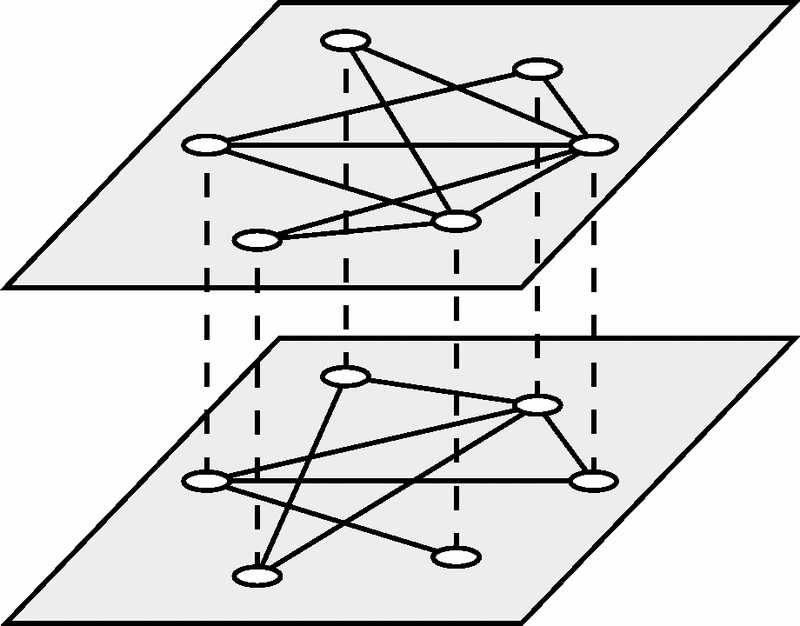
\includegraphics[width = 0.7 \linewidth]{plots/multiplex_network.png}
\end{center}
\end{column}
\end{columns}

In theory, each relationship can be oriented or not. 
\end{frame}

%-------------------------------------------------------------------
   \begin{frame}{Example  :  multiplex seed exchange network}
 

\begin{itemize}
\item Vertices: homes
\item Network 1: Sorgho exchange
\item Network 2: Mil exchange
\end{itemize}

\end{frame}
 
%-------------------------------------------------------------------
\begin{frame}{Example: coexistence multiplex network}
 
\begin{itemize}
\item Vertices : species 
\item Network 1: dry season coexistence 
\item Network 2: coexistence in the wet season
\end{itemize}
 
\end{frame}
%-------------------------------------------------------------------
   \begin{frame}{Formalization}
 Relationship between $i$ and $j$ described by two indicators : 
$$ X_{ij} = (X^1_{ij}, X^2_{ij}) \quad \mbox{ with } \quad X^1_{ij} \in \{0.1\}\quad \mbox{ and } \quad X^2_{ij} \in \{0.1\}$$ 

\begin{itemize}
\item If $2$ networks, $ X_{ij}$ can take $4$ possible values. 
\item If $M$ networks, $ X_{ij}$ can take $2^M$ possible values.  
\end{itemize}

\cite{kefi}, \cite{Barbillon2016d}
 \end{frame}
 
%-------------------------------------------------------------------


\begin{frame}{Objective}
\begin{block}{Understand / study the structure of the multiplex network}
\begin{itemize}
\item Do all actors have the same behavior, or can we distinguish actors according to their behavior? 
\item Examples : 
\begin{itemize}
\item groups of highly connected individuals according to network $1$ and no network $2$.
\item groups of highly connected individuals according to the $2$ networks
\end{itemize}
\item For two non-oriented networks: R package \textsf{blockmodels}. \textcolor{dgreen}{Soon in \textsf{sbm}}
\end{itemize}
\end{block}
\end{frame}

%-------------------------------------------------------------------

 
\begin{frame}{Researcher advisory networks}
\begin{itemize}
\item Level 1: exchange of advice between researchers
\item Level 2: Relationships through laboratories
\end{itemize}
 
 \textbf{Results}
 
\begin{tabular}{cc} 
  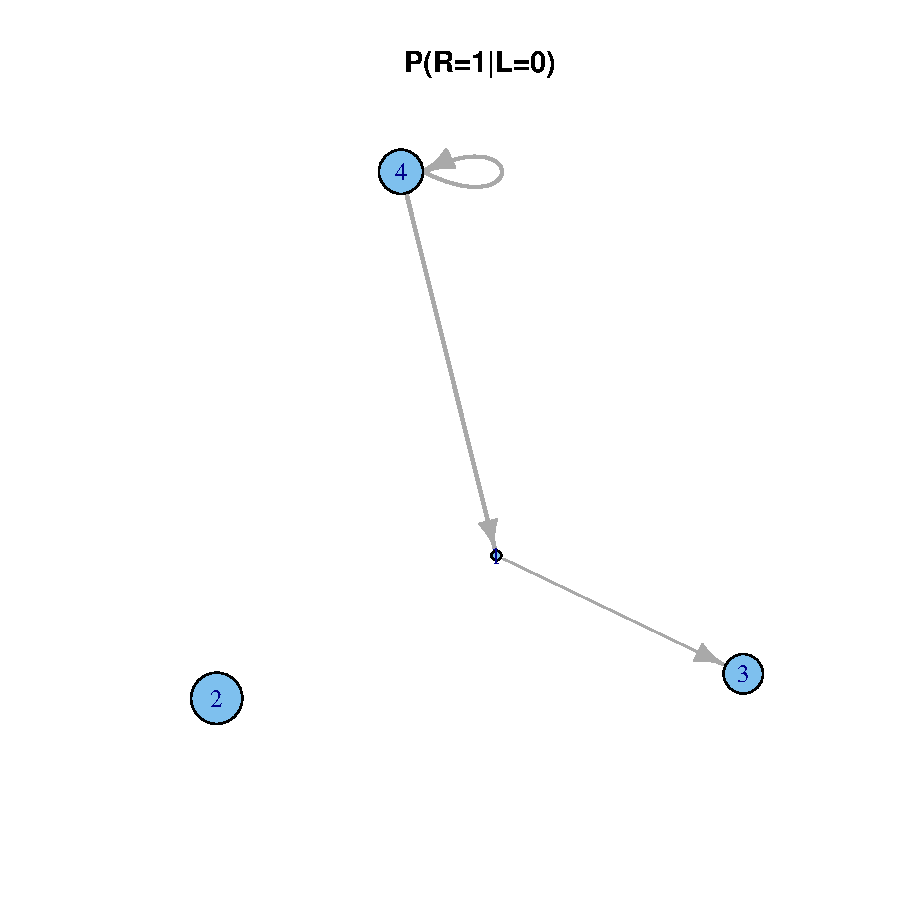
\includegraphics [width = 5cm]{plots/pRL0.pdf} &
 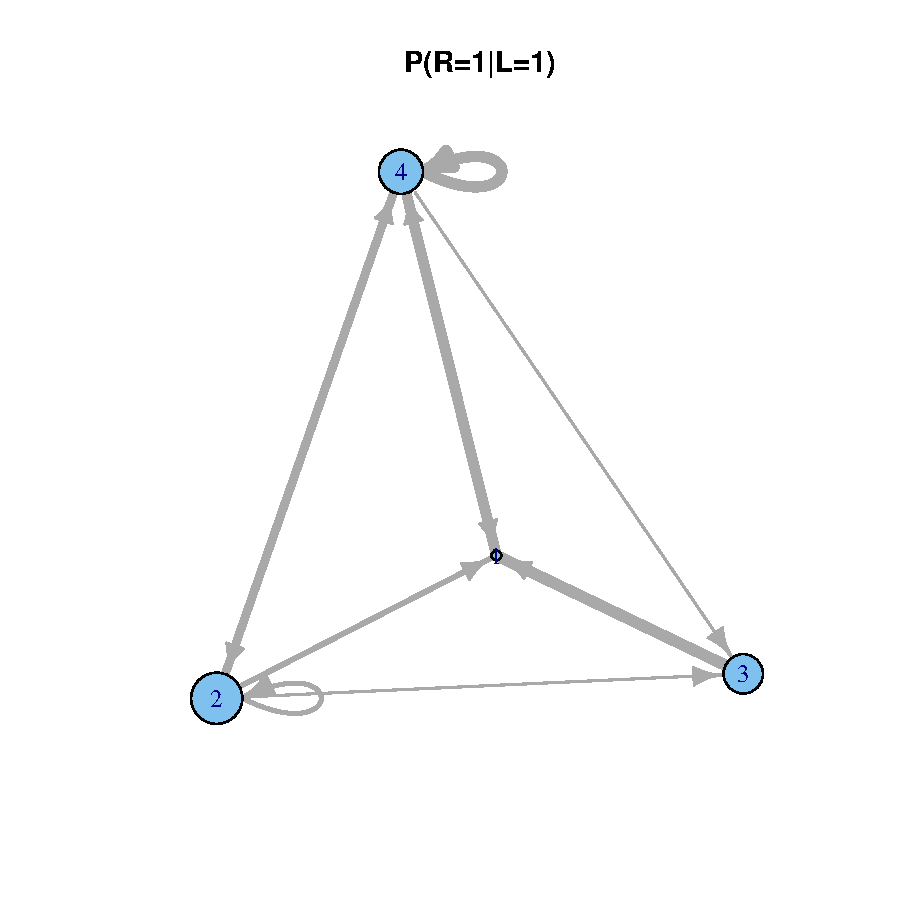
\includegraphics [width =5cm]{plots/pRL1.pdf}
\end{tabular}

\end{frame}

%-------------------------------------------------------------------


\begin{frame}{What you don't do with a multiplex network}
\begin{itemize}
\item If we consider the multiplex version of the network, we don't want to "compare networks". 
\item Considering the multiplex version is really considering that the relationship is \emph{\textcolor{dgreen}{multiple or complex}}. 
\end{itemize}

\end{frame}
%-------------------------------------------------------------------------------
\section{Multipartite networks}


\subsection[Multipartite data]{The type of data we are talking about}


\begin{frame}{Multipartite networks}

 
\begin{block}{Definition}
We talk about multipartite network if the vertices are divided into \textbf{\textcolor{dgreen}{several}} subsets in advance. 
\end{block}


  From bipartite  ...      
\begin{minipage}[t]{0.2\linewidth}
% Bipartite
\begin{tikzpicture}[
  mynoder/.style={draw,circle,text width=0.5cm,fill = red,align=center,scale=0.6},
  mynodeg/.style={draw,circle,text width=0.5cm,align=center, fill = green,scale=0.6},
 ]

\node[mynoder] (R1) {$1$};
\node[mynoder, below=0.1 cm of R1] (R2) {$2$};
 \node[mynoder, below=0.1 cm of R2] (R3) {$3$};
 \node[mynoder, below=0.1 cm of R3] (R4) {$4$};
 \node[mynoder, below=0.1 cm of R4] (R5) {$5$};
 \node[mynoder, below=0.1 cm of R5] (R6) {$6$};
 
\node[mynodeg, right =1 cm of R1] (G1) {$1$};
\node[mynodeg, below=0.1 cm of G1] (G2) {$2$};
 \node[mynodeg, below=0.1 cm of G2] (G3) {$3$};
 \node[mynodeg, below=0.1 cm of G3] (G4) {$4$};
 \node[mynodeg, below=0.1 cm of G4] (G5) {$5$};

\path[thick]
(R1) edge (G2)
(R2) edge (G3) 
(R2) edge (G4)
(R4) edge (G1)
(R4) edge (G5)
(R6) edge (G5);

\end{tikzpicture}
\end{minipage} 


\end{frame}

%-------------------------------------------------------------------------------
\begin{frame}{... to multipartite}
% Multipartite
\begin{minipage}[t]{0.5\linewidth}
\centering
\begin{tikzpicture}[
  mynoder/.style={draw,circle,text width=0.5cm,fill = red,align=center,scale=0.6},
  mynodeg/.style={draw,circle,text width=0.5cm,align=center, fill = green,scale=0.6},
  mynodeb/.style={draw,circle,text width=0.5cm,align=center, fill=cyan,scale=0.6},
mynodey/.style={draw,circle,text width=0.5cm,align=center, fill=yellow,scale=0.6}
]
\foreach \a in {1,2,...,5}{
\node[mynoder] at ({90/6 * (\a)}:  3cm) (R\a) {$\a$};
}
\foreach \a in {1,2,...,6}{
\node[mynodeb] at ({90 + 90/6 * (\a-1)}:  3cm) (B\a) {$\a$};
}
 

\node[mynodeg, below right  = 0.5 cm of B6] (G1) {$1$};
\node[mynodeg, right =0.5  cm of G1] (G2) {$2$};
 \node[mynodeg,right =0.5  cm of G2] (G3) {$3$};
 \node[mynodeg,right =0.5  cm of  G3] (G4) {$4$};
 \node[mynodeg, right =0.5  cm of G4] (G5) {$5$};

\node[mynodey, below = 0.5 cm of G1] (Y1) {$1$};
\node[mynodey, right =0.5  cm of Y1] (Y2) {$2$};
 \node[mynodey,right =0.5  cm of Y2] (Y3) {$3$};
 \node[mynodey,right =0.5  cm of  Y3] (Y4) {$4$};
 \node[mynodey, right =0.5  cm of Y4] (Y5) {$5$};
 \path[thick]
(R2) edge (G3) 
(R3) edge (G5) 
(R2) edge (G4)
(R4) edge (G1)
(R4) edge (G5);



\path[thick]
(G1) edge [dashed] (B1)
(G2) edge [dashed] (B4)
(G4) edge [dashed] (B4)
(G4) edge [dashed] (B5)
(G5) edge [dashed] (B3);

\path[thick]
(G1) edge (Y1)
(G2) edge (Y4) 
(G2) edge (Y3)
(G4) edge (Y2)
(G4) edge (Y1);



\end{tikzpicture}
    \end{minipage}\hfill
\begin{minipage}[t]{0.3\linewidth}
\centering
\begin{tikzpicture}[
  mynoder/.style={draw,circle,text width=0.5cm,fill = red,align=center,scale=0.6},
  mynodeg/.style={draw,circle,text width=0.5cm,align=center, fill = green,scale=0.6},
  mynodeb/.style={draw,circle,text width=0.5cm,align=center, fill=red,scale=0.6}
]
%
%\node[mynoder] (R1) {$1$};
%\node[mynoder, right=0.1 cm of R1] (R2) {$2$};
% \node[mynoder, right=0.1 cm of R2] (R3) {$3$};
% \node[mynoder, right=0.1 cm of R3] (R4) {$4$};
% \node[mynoder, right=0.1 cm of R4] (R5) {$5$};
% \node[mynoder, right=0.1 cm of R5] (R6) {$6$};
 
\node[mynodeg, below =1 cm of R1] (G1) {$1$};
\node[mynodeg, right=0.1 cm of G1] (G2) {$2$};
 \node[mynodeg, right = 0.1 cm of G2] (G3) {$3$};
 \node[mynodeg, right=0.1 cm of G3] (G4) {$4$};
 \node[mynodeg, right=0.1 cm of G4] (G5) {$5$};

\node[mynodeb, below =1 cm of G1] (B1) {$1$};
\node[mynodeb, right =0.1 cm of B1] (B2) {$2$};
 \node[mynodeb, right =0.1 cm of B2] (B3) {$3$};
 \node[mynodeb, right =0.1 cm of B3] (B4) {$4$};
 \node[mynodeb, right=0.1 cm of B4] (B5) {$5$};
 \node[mynodeb, right=0.1 cm of B5] (B6) {$6$};

%\path[thick]
%(R1) edge (G2)
%(R2) edge (G3) 
%(R2) edge (G4)
%(R4) edge (G1)
%(R4) edge (G5)
%(R6) edge (G5);


\path[thick]
(G1) edge (B1)
(G2) edge (B4) 
(G2) edge (B2)
(G4) edge (B6)
(G4) edge (B3)
(G5) edge (B6);


\path[->] 
(B1) edge [bend right = 70] (B2)
(B3) edge [bend right = 70] (B5)
(B5) edge [bend left = 80] (B1)
(B6) edge [bend left = 70] (B4);
\end{tikzpicture}
    \end{minipage}

 


\end{frame}
%---------------------------------------------------------------------------------------------------------------------------------------


\begin{frame}{Ecology example: super multipartite network}

\centering
  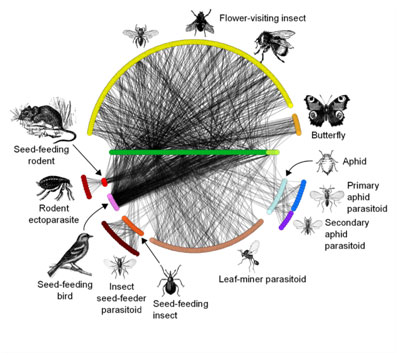
\includegraphics [width = 0.7 \linewidth]{plots/multipartite_super.jpg}
 
\end{frame}
%---------------------------------------------------------------------------------------------------------------------------------------


\begin{frame}{Example in ecology: mutualist relations between animals and plants}

\cite{Dattilo}
 
 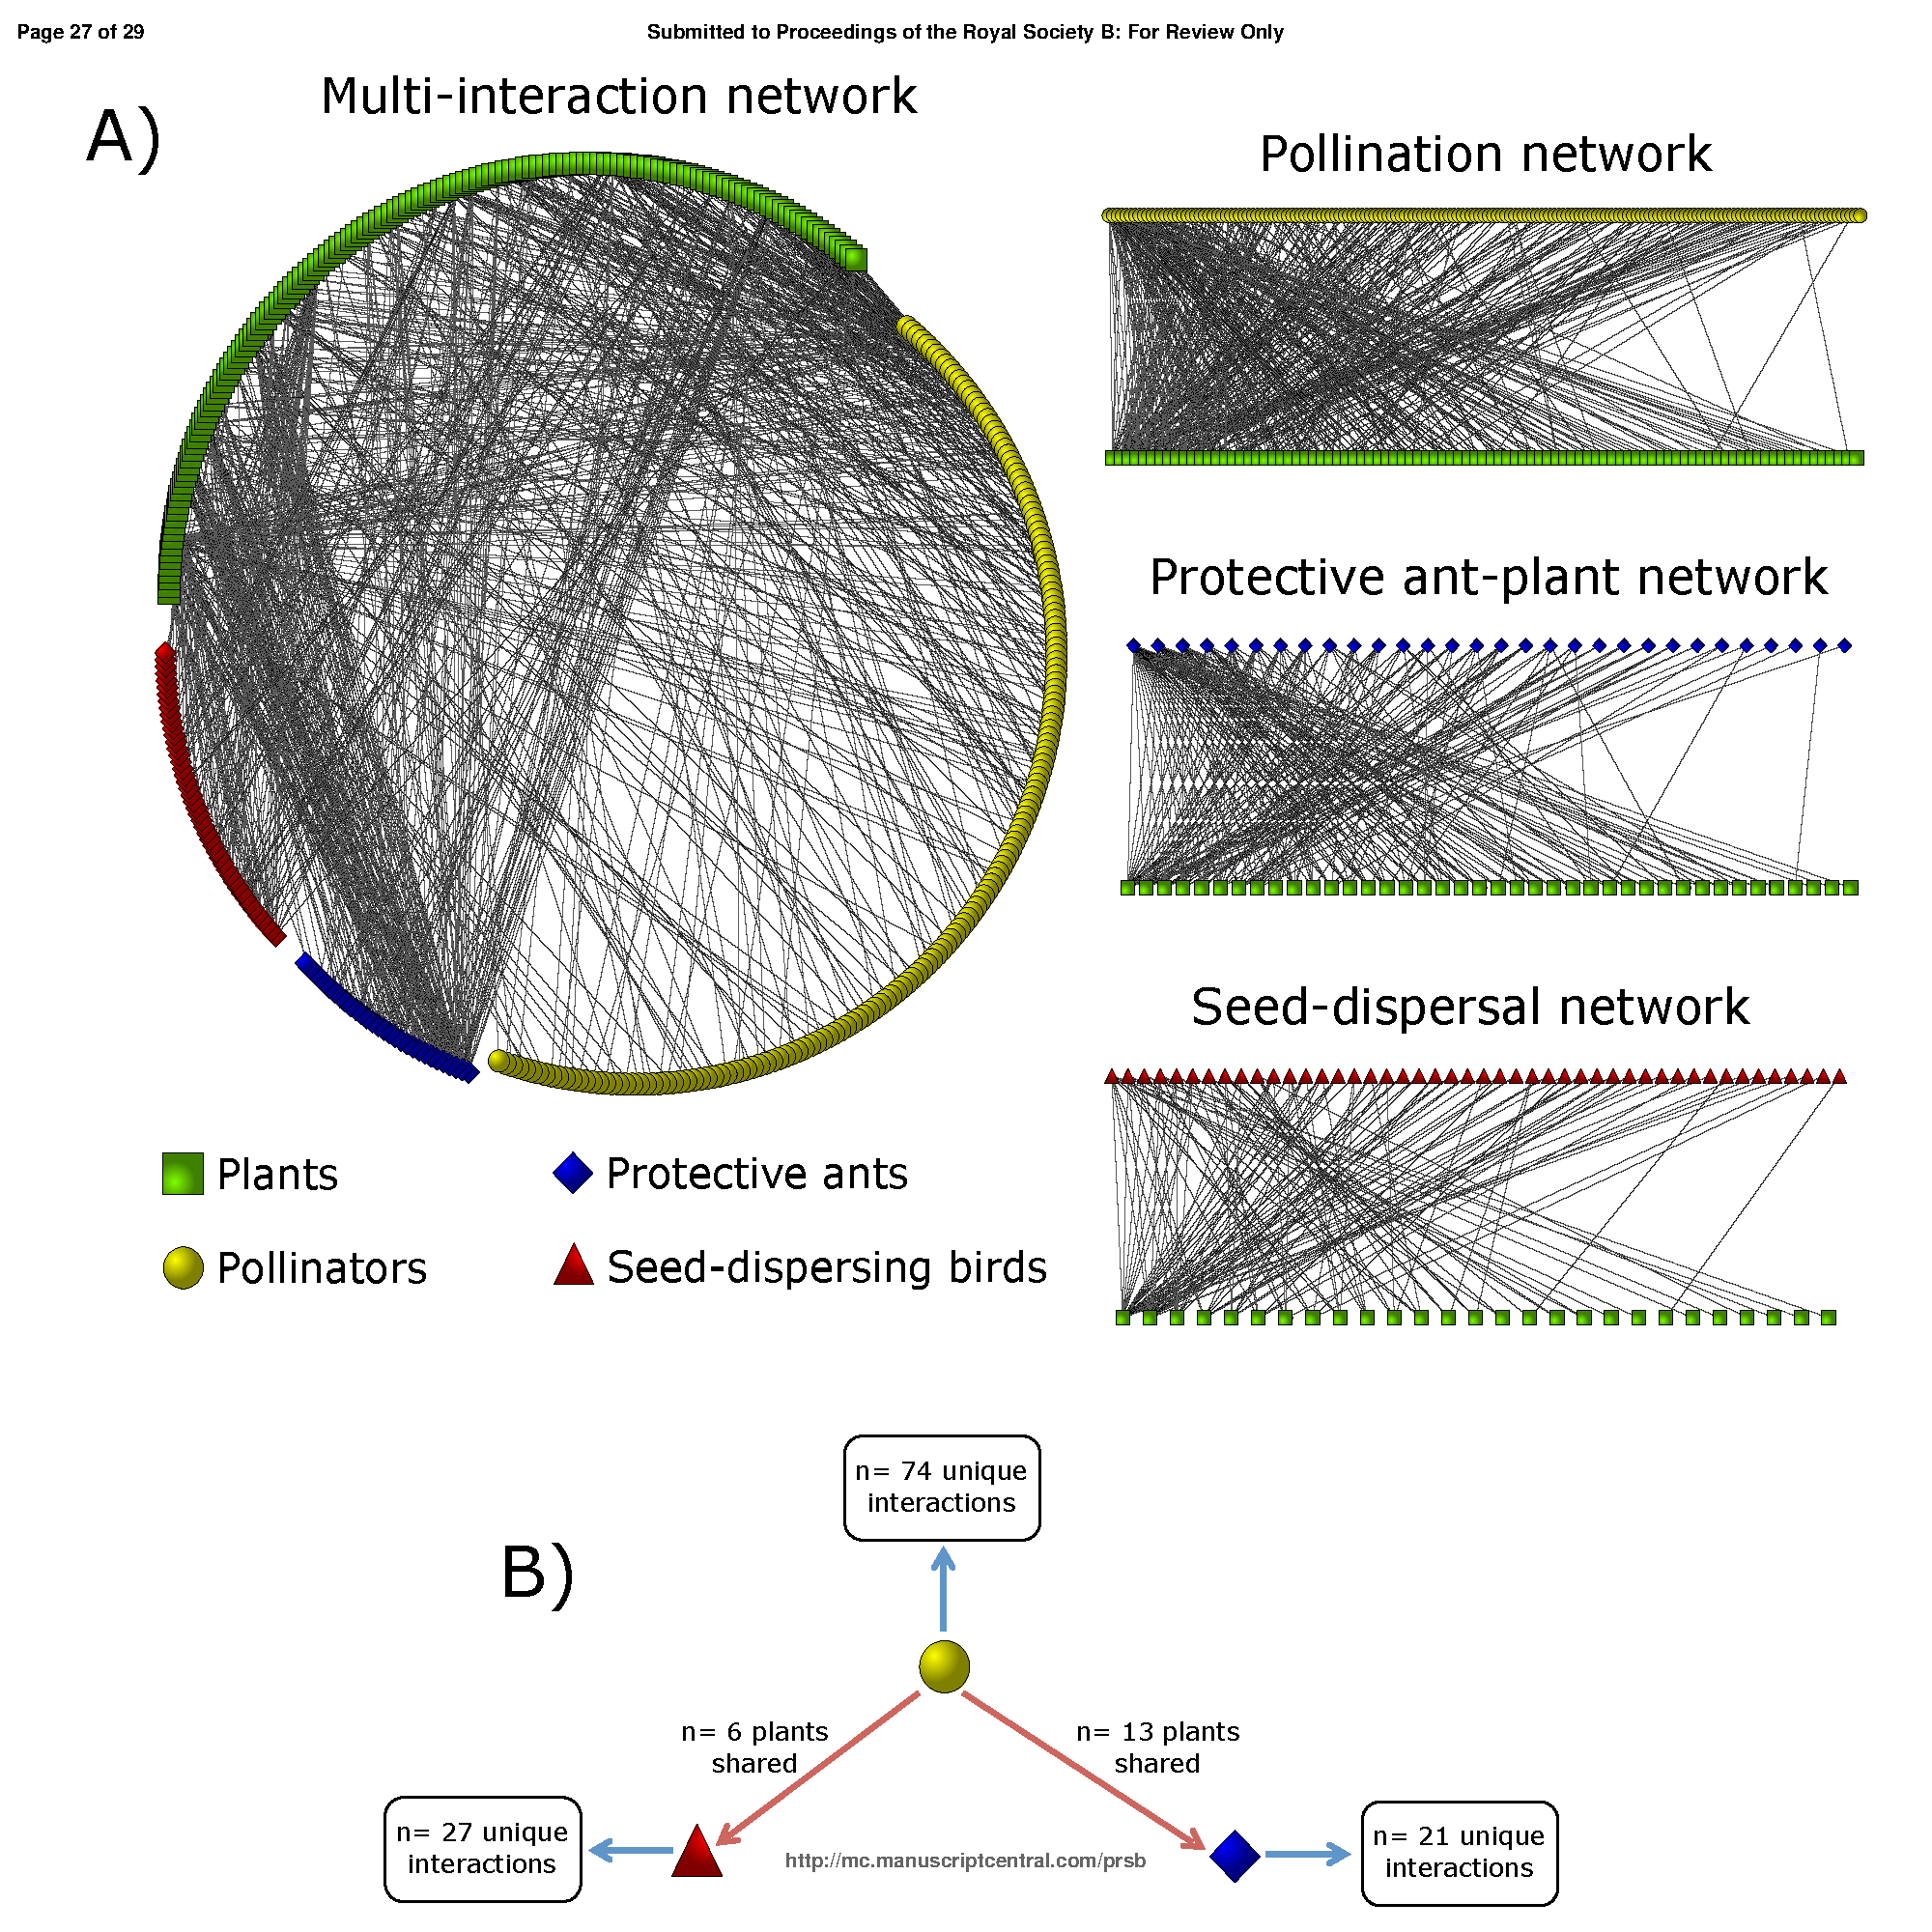
\includegraphics [width = \linewidth]{plots/network_dattilo.pdf}
 
\end{frame}





%--------------------------------------------------------------------------------- 
\begin{frame}{Example in ecology}
\begin{itemize}
 \item Vertices
 \begin{itemize}
 \item Plants ,  Ants,  Seed dispersing birds, Pollinators 
\end{itemize}
\item Interactions : 
\begin{itemize}
 \item[]  [Plants / ants]  --  [Plants / Seed dispersing birds] --  [Plants / Pollinators] 
\end{itemize}
\item 3 bipartite graphs 
\begin{itemize}
\item \textbf{Vertices/ nodes}: plants and animals (divided into functional groups \textcolor{dgreen}{ $\Leftrightarrow$ multipartite graph}) 
\item \textbf{Edge} : if animal seen interacting with plant
\end{itemize}
\item[\textcolor{dgreen}{$\Leftrightarrow$}] 3 rectangular matrices (called \emph{incidences}) 

\end{itemize}
\end{frame}


%-------------------------------------------------------------------------------

\begin{frame}{Data in matrices}

  $$X^{1q}_{ij}=\left\{ \begin{array}{cl}1& \mbox{ if animal  $j$ au functional group $q$ has been seen }\\
  & \mbox{ interacting with plant  $i$ }\\ 0 & \mbox{otherwise}\end{array}\right.$$  

$q=2,3,4$. 
\centering 
\begin{tabular}{|c|ccc|ccc|ccc|}
\hline
 \cellcolor{green!25} Plant 1 &&&1&&&&1&1&1\\
 \cellcolor{green!25} Plant 2 &&&1&&&1&&&1\\
 \cellcolor{green!25} \vdots &&$X^{11}_{ij}$&&&$X^{12}_{ij}$&&&$X^{13}_{ij}$&\\
 \cellcolor{green!25} Plant $n_1$ &1&&1&&&1&1&&1\\
\hline
& \cellcolor{blue!14}  \begin{turn}{-90}Ant $1$\end{turn} &\cellcolor{blue!14} $\cdots$& \cellcolor{blue!14}\begin{turn}{-90}Ant ${n_2}$ \end{turn}&  \cellcolor{red!15} \begin{turn}{-90}\footnotesize Seed dispersing bird  $1$\end{turn}&$\cdots$ \cellcolor{red!15} & \cellcolor{red!15}  \begin{turn}{-90} \footnotesize Seed dispersing bird $n_3$\end{turn} & \cellcolor{yellow!25} \begin{turn}{-90}Pollinator $1$\end{turn}& \cellcolor{yellow!25}  $\cdots$ & \cellcolor{yellow!25}  \begin{turn}{-90}Pollinator $n_4$\end{turn}\\
\hline
\end{tabular}

\vspace{1em}


\footnotesize{$X^q_{ij} \in \{0,1\}$  to avoid sampling problems. } 



\end{frame}



%-------------------------------------------------------------------------------
\begin{frame}{Example 2: sociology / ecology}

\begin{itemize}
 \item Relationships between  farmers (seed exchanges ...) 
\item Inventories of plants (species or varieties) cultivated by the farmers of the network 
\item 2 functional groups : 
\begin{itemize}
\item  farmers : group $1$ 
\item Plants: group $2$
\end{itemize}
\item Interactions : 
\begin{itemize}
 \item  farmers /  farmers :  oriented network
 \item homes / Plants : bipartite network
\end{itemize}
\end{itemize}
\end{frame}

 
\cite{thomasExchanges}

%-------------------------------------------------------------------------------
\begin{frame}{Data in matrices for Example 2}

\begin{table}
\centering
\begin{tabular}{|c||ccc||cccc||}
\hline
 \cellcolor{red!15} Farmer  $1$ &&&1&&&&\\
 \cellcolor{red!15} Farmer  $2$ &&&1&&&&1\\
 \cellcolor{red!15} \vdots &&$X^{11}_{ij}$&&&$X^{12}_{ij}$&&\\
 \cellcolor{red!15} Farmer $n_1$ &1&&1&&&&1\\
\hline
\hline
& \cellcolor{red!15}  \begin{turn}{-90}Farmer $1$\end{turn} &\cellcolor{red!15} $\cdots$& \cellcolor{red!15}\begin{turn}{-90}Farmer  ${n_1}$ \end{turn}&  \cellcolor{green!25} \hspace{1em}\begin{turn}{-90} Plant  $1$\end{turn}&\cellcolor{green!25} $\cdots$ &$\cdots$ \cellcolor{green!25} & \cellcolor{green!25}  \begin{turn}{-90}  Plant$n_2$\end{turn}\\
\hline
\end{tabular}
\end{table}
\end{frame}

%------------------------------------------------------------------------------ 


\begin{frame}{Objectives}

\begin{block}{Aim}
Identify subgroups of each functional group sharing the same interaction characteristics and simultaneously taking into account all the matrices. 
\end{block}

\begin{block}{Existing solutions}
\begin{itemize}
\item Calculate modularity
\begin{itemize}
\item Detecting communities: making subgroups of individuals who connect more within the subgroup than outside it. 
\item In general, people do it separately on each type of interaction and then compare the results between them. 
\end{itemize}
\end{itemize}
\end{block}
\begin{block}{Proposal}
Use extensions of the Latent Block Models (LBM) and Stochastic Block Models (SBM) to propose a classification of individuals/agents based on the set of observations.
\end{block}
\end{frame}




%%-------------------------------------------------------------------------------


\subsection{Modeling a collection of matrices}

%-------------------------------------------------------------------------------
\begin{frame}{Data formatting}
\begin{itemize}
\item $Q$ functional groups. 
\item Each functional group $q$ is of size $n_q$. 
\item \textbf{Data} : a collection of matrices (of adjacency or incidence) representing the relationships within and/or between functional groups: 
\begin{itemize}
\item $\mathcal{E}$ = list of pairs $(q,q')$ for which a matrix of interaction between functional groups $q$ and $q'$ is observed. 
\item $\bX = \{X^{q'}, (q,q') \in \mathcal{E}\}$ where $X^{q'}$ is a matrix of size $n_q \times n_{q'}$. 
\item If $q=q'$ matrix of adjacency, symmetrical or not
\item If $q \neq q'$, incidence matrix, bipartite graph
\end{itemize}
\end{itemize}

\begin{block}{Examples}
\begin{itemize}
\item Example 1: $1 =$ plants, $2=$ ants, $3=$ birds, $4=$ pollinators

\item Example 2: $1 =$ farmers, $2=$ plants 
  
\end{itemize}
\end{block}
\end{frame}


%-------------------------------------------------------------------------------

\begin{frame}{Latent variable probabilistic model}

\begin{itemize}
\item In the spirit of LBM / SBM: mixing model to model edges
\item Each functional group of nodes (or vertices) $q$ is divided into $K_q$ blocks.  
\item $\forall q=1\dots Q$, $Z^q_i=k$ if the entity $i$ of the functional group $q$ belongs to the block $k$. 
\end{itemize}
 

\begin{block}{Latent variables}
 $(Z^q_i)_{i=1\dots n_q}$ latent, independent random variables: $ \forall k=1\dots K_q$, $\forall i=1\dots n_q$, $ \forall q=1\dots Q$, \begin{equation}\label{eq:mod2}
\P(Z^{q}_i=k) = \pi^{q}_k, \quad
\end{equation}
with $\sum_{k=1}^{K_q}\pi^{q}_k=1$ for all $q=1, \dots Q$.
\end{block}

\end{frame}


%-------------------------------------------------------------------------------
\begin{frame}{Latent variable probabilistic model}


\begin{block}{ 
Conditionally... }
... to latent variables $\boldsymbol{Z}=\{Z^{q}_i, i=1\dots n_q, q=1\dots Q\}$ : 

\begin{equation}\label{eq:mod_new}
X^{q'}_{ij} | Z^{q}_i, Z^{q'}_j \sim_{i.i.d} \mathcal{F}(\alpha^{qq'}_{Z^q_i, Z^{q'}_j})\,.
\end{equation}
\end{block}

\begin{itemize}
\item Law of the interaction phenomenon depends on the $i$ and $j$ membership groups 
\item In the examples, $\mathcal{F} = \mathcal{B}ern$ but other possible laws (Fish...)
\item Special cases
\begin{itemize}
\item If only one functional group and $\Ecal=\{(1,1)\}$: SBM
\item If two functional groups and $\Ecal=\{(1,2)\}$ :  LBM
%\item \color{dgreen} $\Rightarrow$ \color{block}
\end{itemize}
\end{itemize}

\cite{multipartite}
\end{frame}


%--------------------------------------------------------------------------- 
\begin{frame}{Synthetic scheme for plants/insects networks} 
 \begin{center}
        \begin{tikzpicture}
          %% UN GRAPH

          \tikzstyle{every edge}=[-,>=stealth',shorten >=1pt,auto,thin,draw]
          \tikzstyle{every state}=[draw=none,text=white,scale=0.65, font=\scriptsize, transform shape]
          
          \node[draw,text width=2cm] at (1,-0.5) {Pollinators};
                \node[draw,text width=1.2cm] at (5,-0.5){Birds};
                 \node[draw,text width=1.2cm] at (8,-0.5){Ants};
	    \node[draw,text width=1.2cm] at (4,5.5) {Plants};	
	\tikzstyle{every node}=[fill=yellow!40!orange]  	
          
          
          % premier cluster de pollinisateurs
          \node[state] (P1) at (-1,0.5) {1};
          \node[state] (P2) at (0,0.5) {2};
          \node[state] (P3) at (1,0.5) {3};


       % deuxième cluster de pollinisateurs
          \node[state] (P4) at (2,0.5) {5};
          \node[state] (P5) at (3,0.5) {6};

          
	% premier cluster de oiseaux
	  \tikzstyle{every node}=[fill=blue!80!black]
          \node[state] (O1) at (4,0.5) {1};
          \node[state] (O2) at (5,0.5) {2};
                    
          	% deuxième cluster de oiseaux
	  \tikzstyle{every node}=[fill=blue!80!black]
          \node[state] (O3) at (6,0.5) {3};
          
          
          % premier cluster de fourmis
	  \tikzstyle{every node}=[fill=red!80!black]
          \node[state] (F1) at (7,0.5) {1};
          \node[state] (F2) at (8,0.5) {2};
                    
          	% deuxième cluster de fourmis
	  \tikzstyle{every node}=[fill=red!80!black]
          \node[state] (F3) at (9,0.5) {3};
           \node[state] (F4) at (10,0.5) {3};
          
          
          
  
  	% troisième cluster 
  	\tikzstyle{every node}=[fill=green!50!black]
  	\node[state] (PL1) at (0,4.5) {1};
          \node[state] (PL2) at (1,4.5) {2};
  	  \node[state] (PL3) at (2,4.5) {3};
  	   \node[state] (PL4) at (3,4.5) {4};
  	  
  	 % quatrième cluster 
  	   \tikzstyle{every node}=[fill=green!50!black]
  	% troisieme cluster
          \node[state] (PL5) at (4,4.5) {5};
          \node[state] (PL6) at (5,4.5) {6};
  	\node[state] (PL7) at (6,4.5) {7};
  	 \node[state] (PL8) at (7,4.5) {8};
  	 \node[state] (PL9) at (8,4.5) {9};
          \end{tikzpicture}
        \end{center}
 \end{frame}
 
 
 
%--------------------------------------------------------------------------- 
\begin{frame}{Synthetic scheme for plants/insects networks} 
 \begin{center}
        \begin{tikzpicture}
          %% UN GRAPH

          \tikzstyle{every edge}=[-,>=stealth',shorten >=1pt,auto,thin,draw]
          \tikzstyle{every state}=[draw=none,text=white,scale=0.65, font=\scriptsize, transform shape]
          
          
          \node[draw,text width=2cm] at (1,-0.5) {Pollinators};
                \node[draw,text width=1.2cm] at (5,-0.5){Birds};
                 \node[draw,text width=1.2cm] at (8,-0.5){Ants};
	    \node[draw,text width=1.2cm] at (4,5.5) {Plants};	
	\tikzstyle{every node}=[fill=yellow!40!orange]  	
          
          
          % premier cluster de pollinisateurs
          
          	\tikzstyle{every node}=[fill=yellow!10!orange]  
          \node[state] (P1) at (-1,0.5) {1};
          \node[state] (P2) at (0,0.5) {2};
          \node[state] (P3) at (1,0.5) {3};


       % deuxième cluster de pollinisateurs
       	\tikzstyle{every node}=[fill=yellow!60!orange]  
          \node[state] (P4) at (2,0.5) {5};
          \node[state] (P5) at (3,0.5) {6};

          
	% premier cluster de oiseaux
	  \tikzstyle{every node}=[fill=blue!40!black]
          \node[state] (O1) at (4,0.5) {1};
          \node[state] (O2) at (5,0.5) {2};
                    
          	% deuxième cluster de oiseaux
	  \tikzstyle{every node}=[fill=blue!90!black]
          \node[state] (O3) at (6,0.5) {3};
          
          
          % premier cluster de fourmis
	  \tikzstyle{every node}=[fill=red!60!black]
          \node[state] (F1) at (7,0.5) {1};
          \node[state] (F2) at (8,0.5) {2};
                    
          	% deuxième cluster de fourmis
	  \tikzstyle{every node}=[fill=red!90!black]
          \node[state] (F3) at (9,0.5) {3};
          
           \node[state] (F4) at (10,0.5) {4};
          
          
          
  
  	%premier  cluster de plantes 
  	\tikzstyle{every node}=[fill=green!50!black]
  	\node[state] (PL1) at (0,4.5) {1};
          \node[state] (PL2) at (1,4.5) {2};
  	  \node[state] (PL3) at (2,4.5) {3};
  	   \node[state] (PL4) at (3,4.5) {4};
  	  
  	 %deuxième   cluster de plantes 
  	   \tikzstyle{every node}=[fill=green!30!black]
  	 
          \node[state] (PL5) at (4,4.5) {5};
          \node[state] (PL6) at (5,4.5) {6};
  	\node[state] (PL7) at (6,4.5) {7};
  	%premier  cluster de plantes 
  	
  	
  	   \tikzstyle{every node}=[fill=green!90!black]
  	 \node[state] (PL8) at (7,4.5) {8};
  	 \node[state] (PL9) at (8,4.5) {9};
  	                              
         
%      
%	\path  (A2) edge [bend right] node[fill=white]
%        	{$\alpha_{\textcolor{yellow!40!orange}{\bullet}\textcolor{green!50!black}{\bullet}}$}
%          (C1) ;
%          \path   (A1) edge [bend right] node[fill=white]
%          {$\alpha_{\textcolor{yellow!40!orange}{\bullet}\textcolor{green!50!black}{\bullet}}$}
%          (C2);
%          
%	\path  (B1) edge [bend right] node[fill=white]
%        	{$\alpha_{\textcolor{green!50!black}{\bullet}\textcolor{blue!50!black}{\bullet}}$}
%          (C2) ;
%       	\path  (B2) edge [bend right] (C1) ;
%	       	\path  (A2) edge [bend left] (D2) ;
       
            \path  (PL7) edge [bend right] (F1) ;
	       	%\path  (PL8) edge [bend left] (F2) ;
	       	       \path  (PL8) edge [bend left] node[fill=white]
        	{$\alpha^ {14}_{\textcolor{green!90!black}{\bullet}\textcolor{red!60!black}{\bullet}}$}(F2) ;
	       	
	       	\path  (PL8) edge [bend left] (O3) ;
	       	
	       	       \path  (PL9) edge [bend right] node[fill=white]
        	{$\alpha^ {12}_{\textcolor{green!90!black}{\bullet}\textcolor{yellow!10!orange}{\bullet}}$}(P3) ;
         	
	       	
	       \path  (PL1) edge [bend right] node[fill=white]
        	{$\alpha^ {12}_{\textcolor{green!50!black}{\bullet}\textcolor{yellow!10!orange}{\bullet}}$}(P1) ;
	     

	       	\path  (PL1) edge [bend left] (P2) ;
	       	\path  (PL2) edge [bend left] (O1) ;
	       	  \path  (PL4) edge [bend right] node[fill=white]
        	{$\alpha^ {13}_{\textcolor{green!50!black}{\bullet}\textcolor{blue!40!black}{\bullet}}$}(O2) ;
	     
	       	%\path  (PL4) edge [bend right] (O2) ;
	       	
	       	   	
	       	
	       	
          % inter cluster
%              \path (B2) edge (B5)
%          (B1) edge (B4);
  
        \end{tikzpicture}
        \end{center}
 \end{frame}
 
 
 \begin{frame}{Résumé}
     \begin{block}{Latent variables}
             Each functional group  $q$  divided into $K_q$ clusters
              \begin{itemize}
     
                \item $\forall q=1\dots Q, \forall i=1\dots n_q$, $Z_i \in \{1,\dots, K_q\}$ Latent variables
              \item $\pi^q_k = \mathbb{P}(Z^q_i = k)$, $\forall i, \forall k,\forall q$
              \item $\sum_{k=1}^{K_q} \pi^q_k=1$
              \item i.i.d. variables
   
       % \item $\alpha_{\textcolor{yellow!40!orange}{\bullet}\textcolor{blue!80!black}{\bullet}} = \mathbb{P}(i
           % \leftrightarrow j | i\in\textcolor{yellow!40!orange}{\bullet},j\in\in\textcolor{blue!80!black}{\bullet})$
              \end{itemize}
            \end{block}
            
             
  \begin{block}{Connection distribution}
  Conditionally to the latent variables : $\forall (q,q') \in \mathcal{E}$
$$
X^{qq'}_{ij} | Z^{q}_i, Z^{q'}_j \sim_{ind} \mathcal{F}(\alpha^{qq'}_{Z^q_i, Z^{q'}_j})\,.
$$
\end{block}
\end{frame}


%-------------------------------------------------------------------------------
\begin{frame}{Dependencies between matrices}


 \begin{itemize}
 
 \item If $K_q = $1 for all $q$ then all the entries of all the matrices are independent random variables: homogeneous connection. 
  \item Otherwise, integration of the random variables \color{dgreen} $\Rightarrow$ \color{black} dependence between the elements of the matrices  
  \item Dependence between matrices %concerning a common functional group
\item \textbf{Consequences} on $\bZ^q | \bX$ 
\begin{itemize}
\item The obtained clustering  depends on all interaction matrices.  
  \item Few simplifications possible
  \end{itemize}
  
  \end{itemize}
  
\end{frame}
%-------------------------------------------------------------------------------
\begin{frame}{DAG for example 1}

\begin{itemize}
\item $1 =$ plants
\item $2 =$ ants
\item $3 =$ farmers
\item $2 =$ cultivated plants

\end{itemize}

 
\centering

\begin{tikzpicture}[
  node distance=1cm and 1cm,
  mynodec/.style={draw,ellipse,text width=1.5cm,align=center},
  mynode/.style={draw,rectangle,text width=1.5cm,align=center},
  mynodep/.style={draw,circle,text width=0.5cm,align=center}
]

\node[mynode] (x12) {$X^{12}$};
\node[mynode, right=0.8 cm of x12] (x13) {$X^{13}$};
\node[mynode,  right=0.8 cm of  x13] (x14) {$X^{14}$};
\node[mynodec, above left=0.5 cm of x12] (z2) {$\bZ^{2}$}; 
\node[mynodec, right=2 cm of z2] (z1) {$\bZ^{1}$};
\node[mynodec,  right=2cm of z1] (z3) {$\bZ^{3}$};
\node[mynodec, below right=0.5cm of x14] (z4) {$\bZ^{4}$};
\path (z3) edge[-latex] (x13)
(z1) edge[-latex] (x12) 
(z1) edge[-latex] (x13) 
(z1) edge[-latex] (x14) 
(z2) edge[-latex] (x12)
(z4) edge[-latex] (x14);
\end{tikzpicture}
 
\end{frame}

%-------------------------------------------------------------------------------

\begin{frame}{DAG pour l'exemple 2}


\begin{itemize}
\item $1 =$ farmers
\item $2 =$ species
\end{itemize}

\begin{figure}
\centering


\begin{tikzpicture}[
  node distance=1.5cm and 1cm,
  mynodec/.style={draw,ellipse,text width=1.5cm,align=center},
  mynode/.style={draw,rectangle,text width=1.5cm,align=center}
]
\node[mynode] (x11) {$X^{11}$};
\node[mynode, right=1 cm of x11] (x12) {$X^{12}$};
\node[mynodec, above =1 cm of x11] (z1) {$\bZ^{1}$}; 
\node[mynodec,above =1 cm of x12] (z2) {$\bZ^{2}$};
\path (z2) edge[-latex] (x12)
(z1) edge[-latex] (x12) 
(z1) edge[-latex] (x11);
\end{tikzpicture}

\end{figure}

\end{frame}



\subsection{Inference}

\begin{frame}{Estimation and model selection}

\begin{itemize}
\item Likelihood maximized by an adapted version of the VEM algorithm
\item Numbers of blocks $(K_1, \dots; K_Q)$ chosen with an adapted ICL criterion (penalized likelihood)
\item Method implemented in \textsf{R package sbm}
\end{itemize}

\end{frame}


    %------------------------------------------------------------------------------------------------------
%    \begin{frame}{Résultats en écologie }
%
%Package R : \textsf{Gremlin} qui peut gérer toutes les structures de réseaux multipartites (encodage en réseau de réseaux).  Données binaires ou de comptage.  
% \begin{itemize}
%\item  7 groupes de plantes 
%\item 2 groupes de pollinisateurs
%\item 1 groupe d'oiseaux
%\item 2 groupes de fourmis
%\end{itemize}
%
% \centering  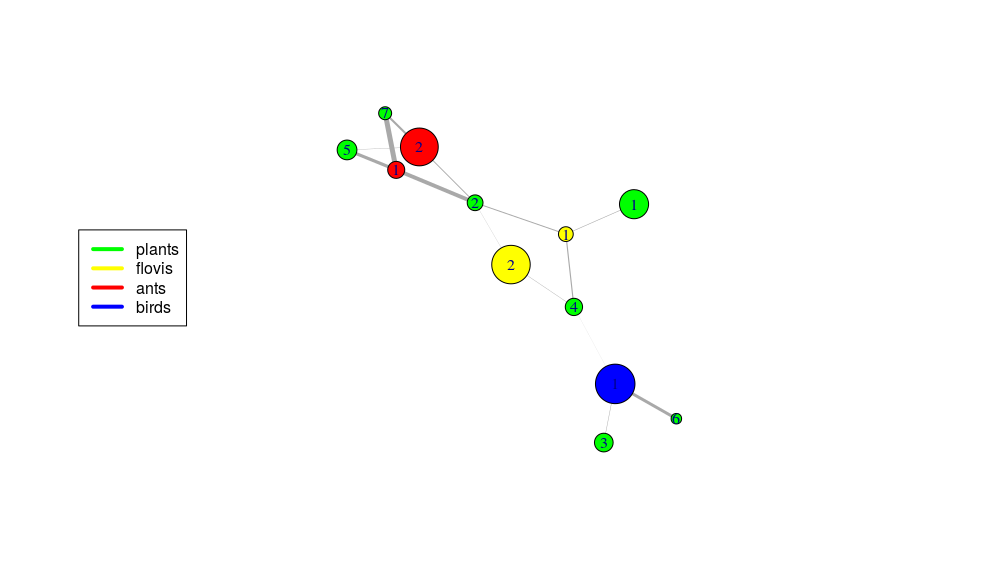
\includegraphics[width =\linewidth]{plots/res_dattilo_MBM.png}
% 
% \end{frame}
%    %------------------------------------------------------------------------------------------------------
%    \begin{frame}{Comparaison à un LBM classique}
%\begin{itemize}
%\item  6 groupes de plantes 
%\item 5 groupes d'animaux
%\end{itemize}
%
% \centering  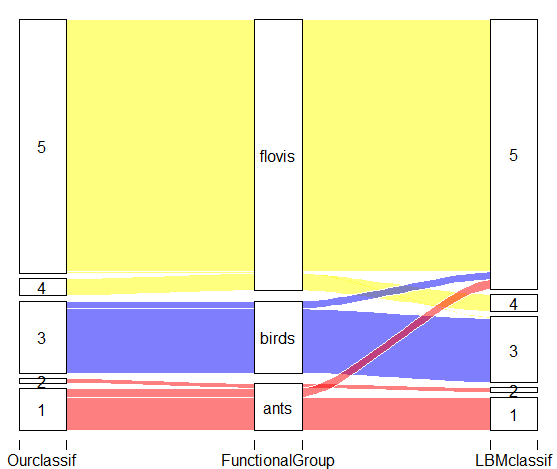
\includegraphics[width =0.8\linewidth]{plots/alluvial_dattilo_animals.png}
% 
% \end{frame} 
%    %------------------------------------------------------------------------------------------------------
%    
% 
%    %------------------------------------------------------------------------------------------------------
%    \begin{frame}{Comparaison à un LBM classique}
%
%
% \centering  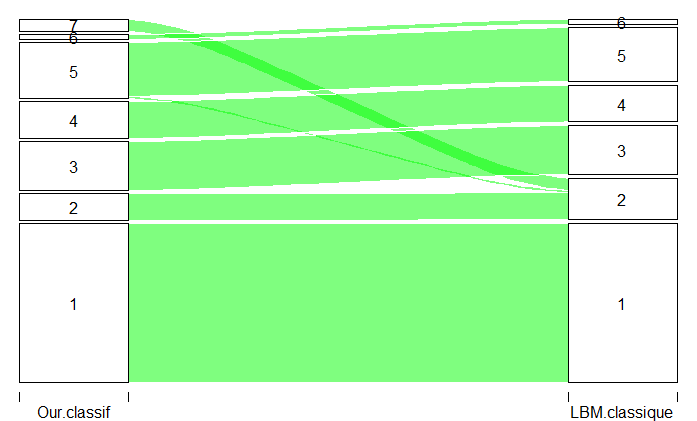
\includegraphics[width =\linewidth]{plots/alluvial_dattilo_plants.png}
% 
% \end{frame} 
% 
     %------------------------------------------------------------------------------------------------------
    
\begin{frame}{Results on data MIRES}

2 groups of crop species, 3 groups of farmers

 \centering  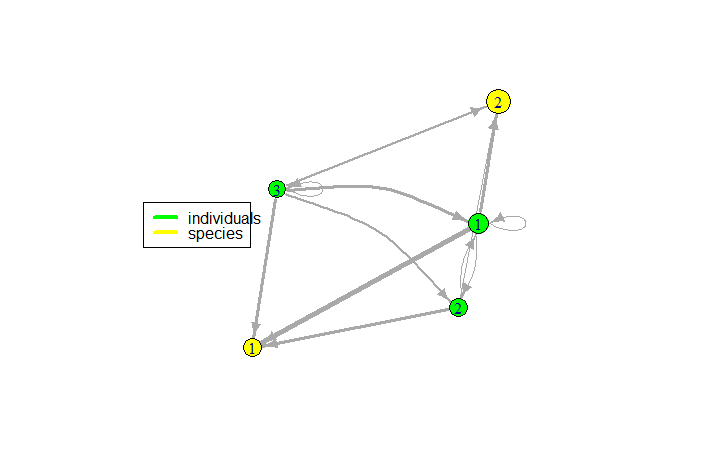
\includegraphics[width =\linewidth]{plots/res_MIRES_MBM.png}



 \end{frame}
 
%------------------------------------------------------------------------------------------------------
    
\begin{frame}{Comparison with a LBM or SBM}


 \centering  

\hspace{-3em}
\begin{minipage}[c]{.46\linewidth}
     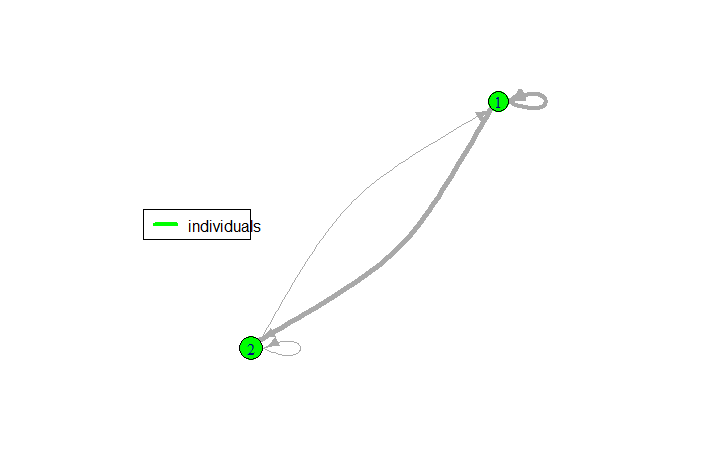
\includegraphics[width = 1.5 \linewidth]{plots/res_MIRES_SBM_individuals.png}
\end{minipage} \hfill
   \begin{minipage}[c]{.46\linewidth}
 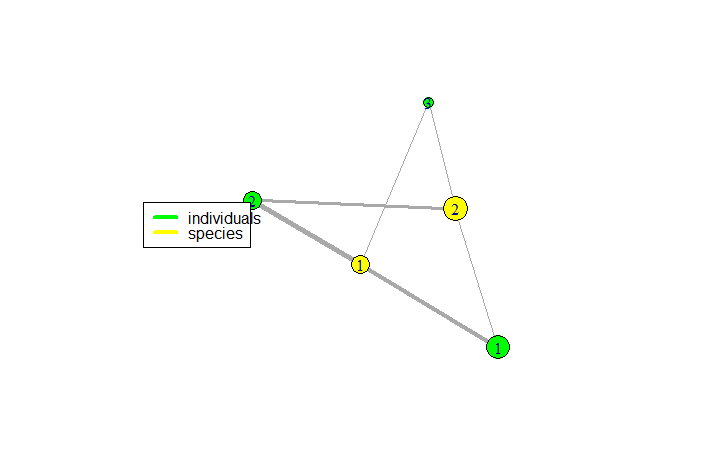
\includegraphics[width = 1.5\linewidth]{plots/res_MIRES_species.png}
   \end{minipage}
   
 \centering  
 \end{frame}
%------------------------------------------------------------------------------------------------------
    
\begin{frame}{Comparison of crop species classifications}

 \centering  

     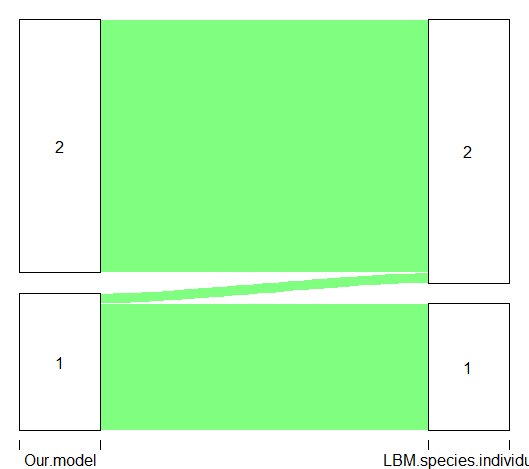
\includegraphics[width = 0.8\linewidth]{plots/alluvial_MIRES_plants.png}

 \end{frame} 
%------------------------------------------------------------------------------------------------------
    
\begin{frame}{Comparison of individual classifications}

 \centering  

     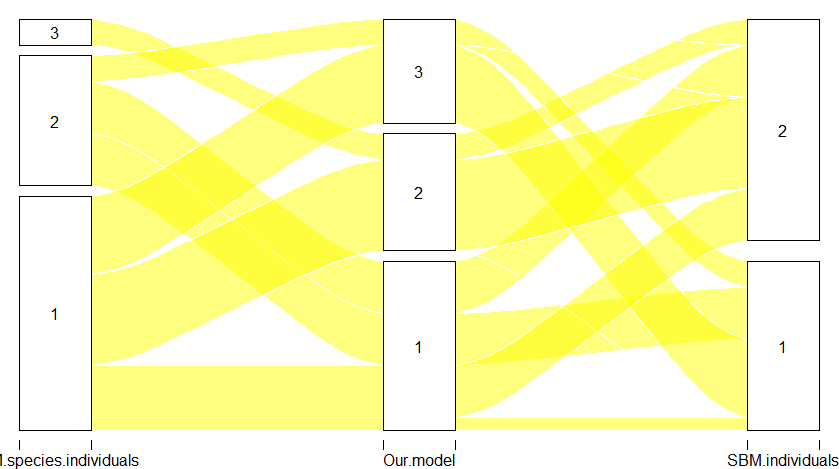
\includegraphics[width = \linewidth]{plots/alluvial_MIRES_individuals.png}



 \end{frame}


%------------------------------------------------------------------------------------------------------
%------------------------------------------------------------------------------------------------------
\section{Multilevel Networks}
 
\begin{frame}{Multilevel networks}
  \begin{block}{Definition}
A multilevel network is said to exist if the vertices are divided into \textbf{\textcolor{dgreen}{several}} subsets in advance and there is a \textbf{\textcolor{dgreen}{hierarchical}} relationship between the vertices.
\end{block}
\vspace{2em}


\begin{columns}
\begin{column}{0.5\textwidth}
\textbf{Example} : 
\begin{itemize}
\item Network of encounters between dogs
\item Network of encounters of their owners
\end{itemize}
\end{column}
\begin{column}{0.5\textwidth} 
 \begin{center}
  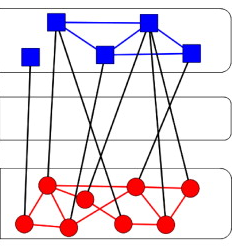
\includegraphics [width = 0.6 \linewidth]{plots/multilevel_network.png}
\end{center}
\end{column}
\end{columns}

Each relationship can be oriented or not. 
\end{frame}
%------------------------------------------------------------------------------------------------------
\begin{frame}{Example in sociology}
\begin{itemize}
\item Informal inter-individual network (counseling, oriented)
\item Formal inter-organizational network (contract, not oriented)
\item Relationship of affiliation of each individual to a single organization
\end{itemize}
 \begin{center}
  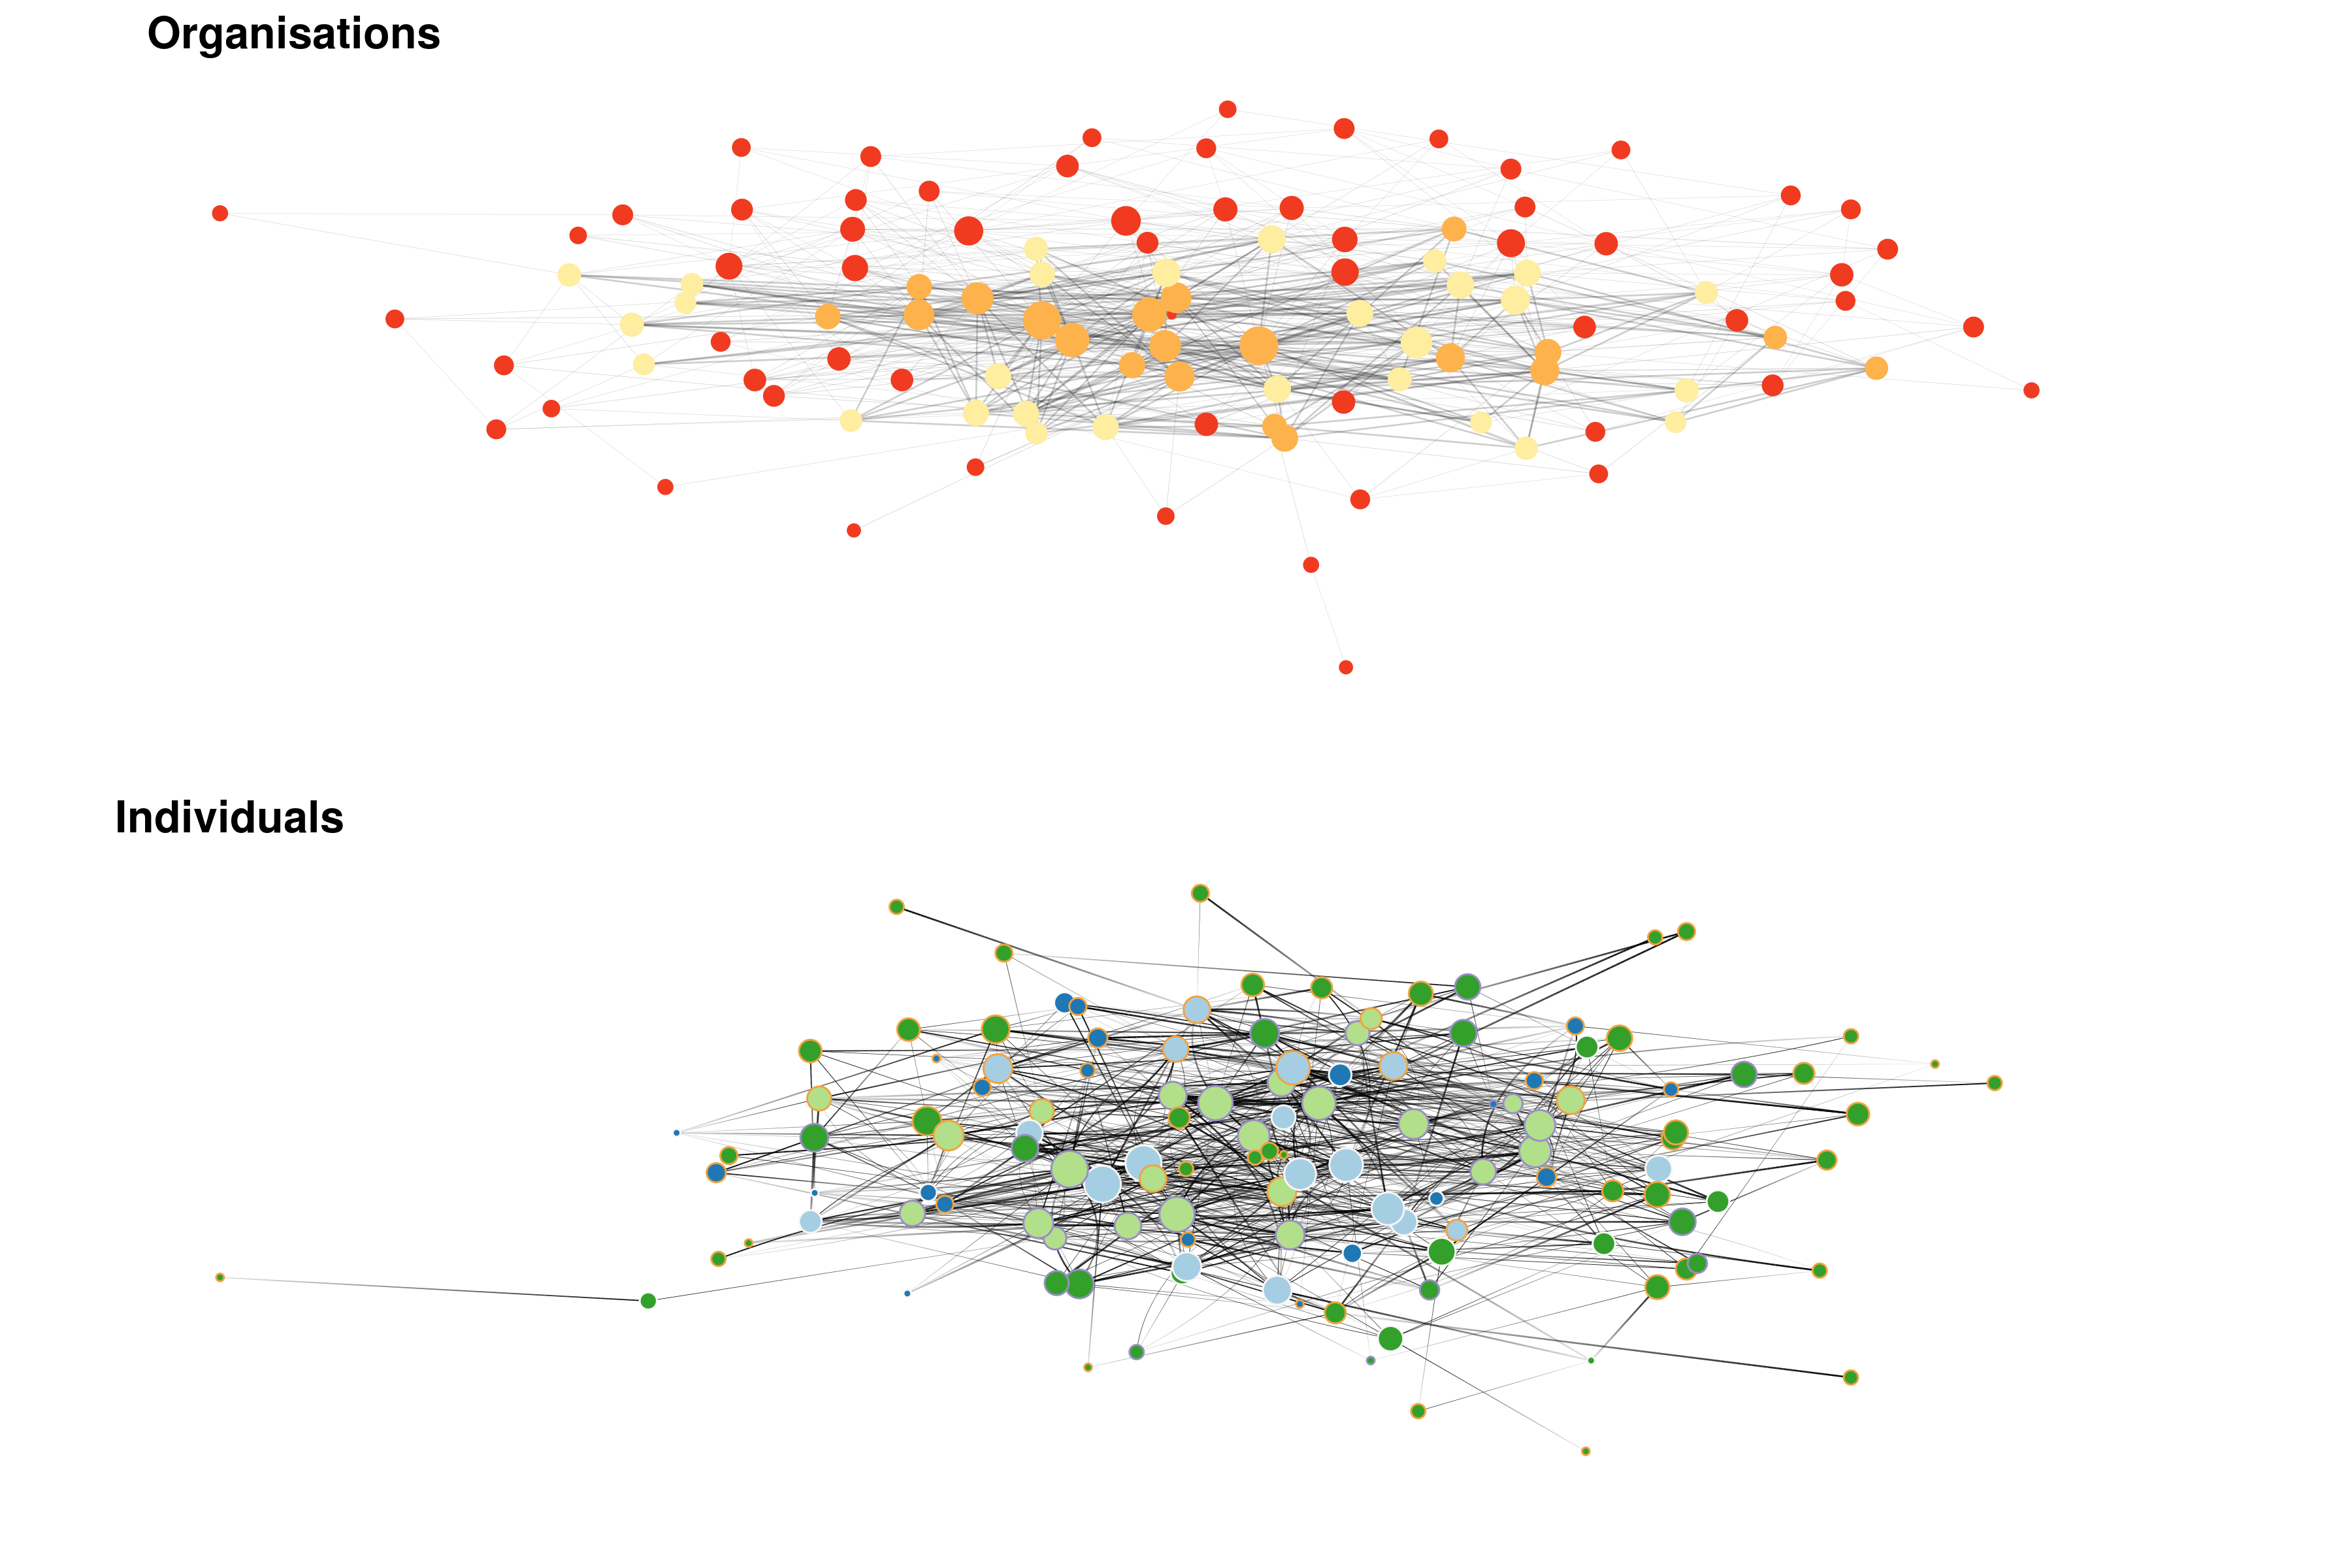
\includegraphics [width = 0.85 \linewidth]{plots/deal_network.png}
  \end{center}
\end{frame}
%------------------------------------------------------------------------------------------------------
\begin{frame}{Objectives}
  \begin{itemize}
    \item Obtain a joint classification of individuals and organizations 
    \item Stating on a dependency of the connection structures between the two levels.
  \end{itemize}


\cite{chabertliddell2019stochastic}

\end{frame}

%------------------------------------------------------------------------------------------------------
\begin{frame}{Results in Sociology}
Package \texttt{R} : \texttt{MLVSBM} which can manage two-level multilevel networks with binary data. 

\begin{itemize}
\item 4 groups of individuals
\item 3 groups of organizations
\item Dependent inter-individual and inter-organizational relationships
\end{itemize}
 \begin{center}
  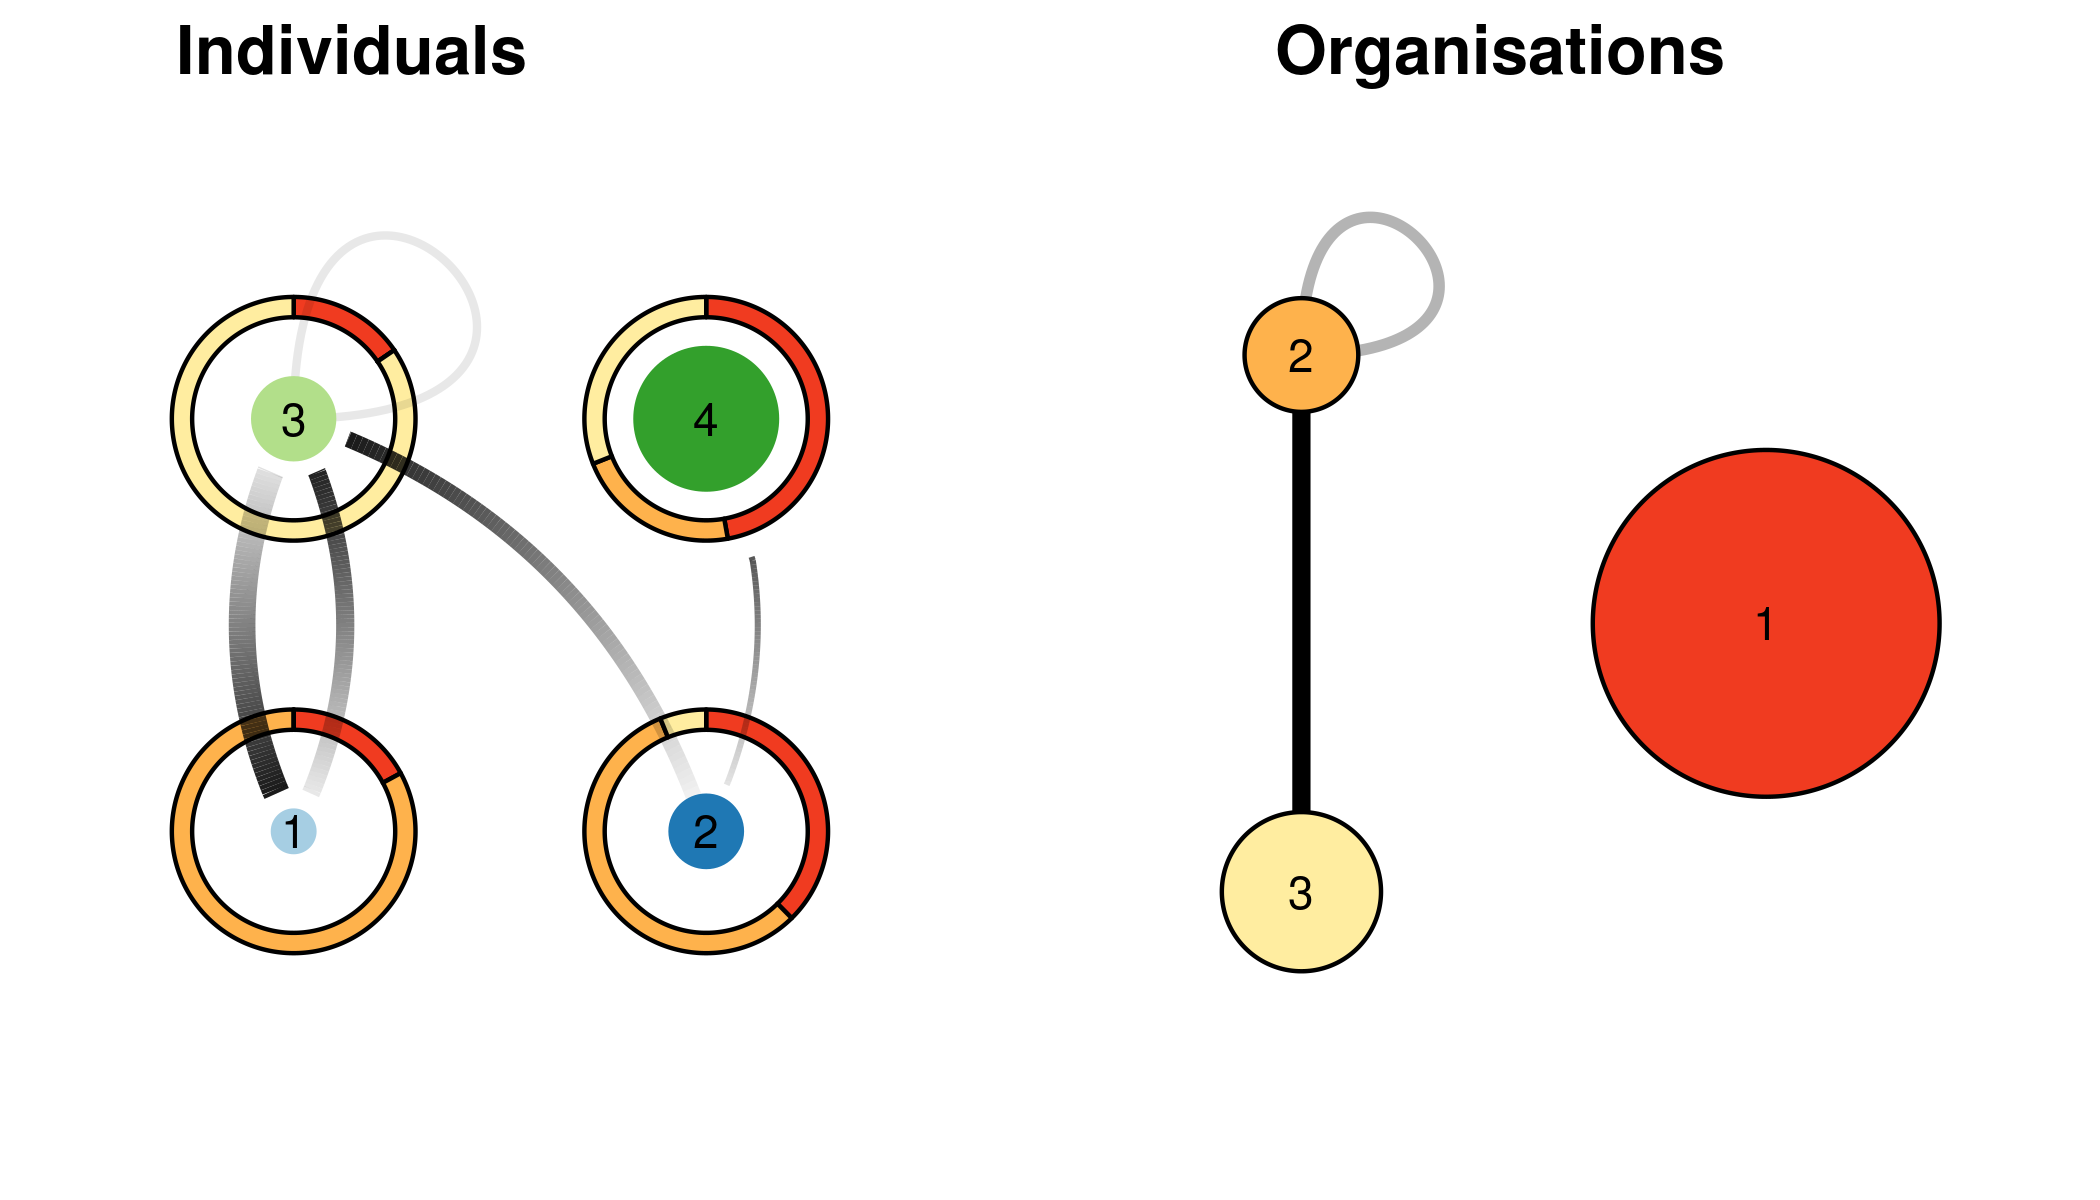
\includegraphics [width = 0.7 \linewidth]{plots/deal_summary_clust.png}
  \end{center}
\end{frame}



%------------------------------------------------------------------------------------------------------
 
    \begin{frame}{Conclusions and perspectives}
 
\begin{block}{Not evoked multiple networks}

\begin{itemize}
\item Dynamic networks: networks that evolve over time. 
\begin{itemize}
\item Either: network photo in discrete times
\item Either: observation of connections in continuous time
\end{itemize}

\item Spatial variation of a network of interest: observation at different locations of the "same" network. 
\end{itemize}
\end{block}


\begin{block}{The evoked networks: multilayer networks}

\begin{itemize}
\item List of networks \emph{multi} that we are able to model and infer
\item Which ones are not included in this catalog? 
\item Does it make sense to take into account several networks at the same time? 
\item Do we prefer comparing networks? How do we compare networks defined on different sets of nodes. 
\end{itemize}

\end{block}
\end{frame}
  
%---------------------------------------------------------------------------------


\begin{frame}[allowframebreaks]{Références}
\bibliographystyle{apalike}
 \small{ 
\bibliography{biblio}}
  \end{frame}
  
  
  
  
%---------------------------------------------------------------------------------



\end{document}

%%%Local Variables:
%%% mode: latex
%%% eval: (TeX-PDF-mode 1)
%%% ispell-local-dictionary: "francais"
%%% eval: (flyspell-mode 1)
%%%End:


